% Pollis drill-down: Compose > Literature Radar, its four pages (Discover Literature, Import References, Browse References
% and Snowball Search Map), what each does and how it works underneath (26 October 2026).
% For users who want the detail, and for whoever maintains Pollis.
% Compile with: latexmk -pdf workflow_literature_radar.tex
% Shared look for the one-page Pollis workflow handouts (same fonts and colours as the brochure).
\documentclass[10pt,a4paper]{article}

\usepackage[a4paper,left=17mm,right=17mm,top=14mm,bottom=16mm,footskip=8mm]{geometry}
\usepackage[T1]{fontenc}
\usepackage[default,semibold]{sourcesanspro}
\usepackage{microtype}
\usepackage{graphicx}
\usepackage[table]{xcolor}
\usepackage{tikz}
\usepackage[most]{tcolorbox}
\usepackage{fontawesome5}
\usepackage{enumitem}
\usepackage{fancyhdr}
\usepackage[hidelinks]{hyperref}

\graphicspath{{images/}}

% ---------------------------------------------------------------- colours (as in the brochure)
\definecolor{navy}{HTML}{1C3A5E}
\definecolor{pblue}{HTML}{3B78B5}
\definecolor{amber}{HTML}{F2B33D}
\definecolor{deepamber}{HTML}{D9902A}
\definecolor{pale}{HTML}{EEF3F9}
\definecolor{ink}{HTML}{2A2F36}
\definecolor{logonavy}{HTML}{173D63}
\definecolor{logodark}{HTML}{C98A1E}
\definecolor{logoamber}{HTML}{F2B446}
\definecolor{logocream}{HTML}{FEEFD2}
\definecolor{soft}{HTML}{5E6773}
\color{ink}

\setlength{\parindent}{0pt}
\setlength{\parskip}{3pt}
\setlist{nosep,leftmargin=*,itemsep=2pt}

\pagestyle{fancy}
\fancyhf{}
\renewcommand{\headrulewidth}{0pt}
\fancyfoot[L]{\footnotesize\color{soft}\textbf{Pollis}\enspace Bright Insights through Statistical Learning, Simulation and Optimisation}
\fancyfoot[R]{\footnotesize\color{soft}github.com/saragga/pollis/releases/latest}

% The Pollis logo, redrawn so it prints sharply at any size
\newcommand{\pollislogo}[1]{%
  \begin{tikzpicture}[x=#1/512,y=-#1/512,baseline=(current bounding box.center)]
    \fill[logonavy] (0,0) rectangle (512,512);
    \fill[logodark] (36,422) -- (104,256) -- (172,422) -- cycle;
    \fill[logoamber] (104,422) -- (203,180) -- (302,422) -- cycle;
    \fill[logocream] (203,422) -- (339,89) -- (476,422) -- cycle;
  \end{tikzpicture}}

% Top of the page: logo, name, kind of document (Workflow unless given, e.g. [Drill-Down]) and its subject;
% then the question and a one-line promise
\newcommand{\workflowhead}[4][Workflow]{%
  \thispagestyle{fancy}%
  \begin{minipage}[c]{13mm}\pollislogo{11mm}\end{minipage}%
  \begin{minipage}[c]{\dimexpr\linewidth-13mm\relax}
    {\color{navy}\Large\bfseries Pollis}\enspace{\color{soft}#1}\hfill
    {\color{deepamber}\small\bfseries\MakeUppercase{#2}}
  \end{minipage}\par\vspace{7mm}
  {\color{navy}\fontsize{22}{26}\selectfont\bfseries #3}\par\vspace{4pt}
  {\color{soft}\large #4}\par\vspace{5mm}}

% A menu path: \menu{Explore}{Access Data Libraries}... is written as \path{Explore \gt Access Data Libraries}
\newcommand{\gt}{\,{\color{deepamber}\bfseries ›}\,}
\newcommand{\menupath}[1]{{\footnotesize\bfseries\color{navy}#1}}

% A screenshot if images/<file> exists, otherwise an orange placeholder that says what to capture
\newlength{\shotheight}\setlength{\shotheight}{43mm}
\newcommand{\stepshot}[2]{%
  \IfFileExists{images/#1}{%
    \tcbox[enhanced, colback=black, colframe=black!70, boxrule=0.4pt, arc=2pt,
      left=0pt,right=0pt,top=0pt,bottom=0pt, boxsep=0pt, halign=center]{%
      \includegraphics[width=\dimexpr\linewidth-1pt\relax,height=\shotheight,keepaspectratio]{#1}}}{%
    \begin{tcolorbox}[enhanced, colback=white, colframe=orange!80, boxrule=0.6pt, arc=2pt,
      height=\shotheight, valign=center, halign=center, left=6pt, right=6pt]
      {\color{orange}\Large\faCamera}\par\smallskip
      {\color{orange}\footnotesize\bfseries Screenshot: #2}\par\smallskip
      {\color{orange!80!black}\scriptsize images/#1}
    \end{tcolorbox}}}

% One step: number, title, menu path, image file, what to capture, what it means
\newcommand{\step}[6]{%
  \begin{tcolorbox}
    {\color{deepamber}\Large\bfseries #1}\enspace{\color{navy}\large\bfseries #2}\par\vspace{1pt}
    \menupath{#3}\par\vspace{4pt}
    \stepshot{#4}{#5}\par\vspace{3pt}
    {\small #6}
  \end{tcolorbox}}

\newenvironment{steps}{%
  \begin{tcbraster}[raster columns=2, raster equal height=rows, raster column skip=4mm,
    raster row skip=4mm, enhanced, colback=pale, colframe=pale, boxrule=0pt, sharp corners,
    left=6pt,right=6pt,top=6pt,bottom=6pt, fontupper=\raggedright]}{\end{tcbraster}}

% Boxes for the bottom of the page
\newtcolorbox{pbox}[2][]{enhanced, colback=pale, colframe=amber, boxrule=0pt,
  leftrule=3pt, sharp corners, left=7pt, right=7pt, top=6pt, bottom=6pt,
  fontupper=\small\raggedright, before upper={{\color{navy}\normalsize\bfseries #2}\par\smallskip}, #1}
\newtcolorbox{nbox}[1][]{enhanced, colback=navy, colframe=navy, boxrule=0pt,
  sharp corners, left=8pt, right=8pt, top=6pt, bottom=6pt, coltext=white,
  fontupper=\small\raggedright, #1}

% A Next Steps item inside the bottom boxes
\newcommand{\nsitem}[2]{\item[\color{deepamber}\faChevronRight] \textbf{#1}: #2}


\usepackage{titlesec}
\usepackage{tabularx}
\usepackage{booktabs}
\usepackage{listings}
\usetikzlibrary{positioning,arrows.meta,fit}

\fancyhf{}
\fancyfoot[L]{\footnotesize\color{soft}\textbf{Pollis}\enspace Drill-down: Literature Radar}
\fancyfoot[R]{\footnotesize\color{soft}\thepage}

\titleformat{\section}{\color{navy}\large\bfseries}{\color{deepamber}\thesection}{0.6em}{}
\titleformat{\subsection}{\color{navy}\normalsize\bfseries}{\color{deepamber}\thesubsection}{0.5em}{}
\titlespacing*{\section}{0pt}{12pt}{4pt}
\titlespacing*{\subsection}{0pt}{8pt}{2pt}
\setlength{\parskip}{4pt}

\lstset{basicstyle=\ttfamily\footnotesize, columns=fullflexible, keepspaces=true, breaklines=true,
  backgroundcolor=\color{pale}, frame=leftline, rulecolor=\color{amber}, framerule=2pt, xleftmargin=6pt,
  framexleftmargin=6pt, aboveskip=4pt, belowskip=4pt, upquote=true, tabsize=2}

\usepackage{xurl}
\newcommand{\file}[1]{{\small\nolinkurl{#1}}}
\newcolumntype{L}{>{\raggedright\arraybackslash}X}

\begin{document}

\workflowhead[Drill-Down]{Literature Radar}
  {Finding the literature, and keeping it}
  {Discover Literature, Import References, Browse References and Snowball Search Map: every control of the four pages,
   what each asks of OpenAlex and Semantic Scholar, how the answers are merged and ranked, and where what you keep is
   written.}

\begin{nbox}
{\color{amber}\bfseries Drill-down.}\enspace
A look under the surface of what the Guide describes in \emph{Literature Radar} and \emph{Snowball Search Map}. It is
for anyone who wants to know why a search returns what it returns, and for whoever maintains Pollis
(\S\ref{sec:where} and \S\ref{sec:open} are for them). It describes the state of 26 October 2026.
\end{nbox}

\tableofcontents

\section{The four pages in one table}

\menupath{Compose\gt Literature Radar} has four items. Two bring works in, one looks after what you kept, and one
follows citations from the works you know to the works you do not.

\begin{center}\small
\renewcommand{\arraystretch}{1.25}
\begin{tabularx}{\linewidth}{@{}p{0.15\linewidth}LLLL@{}}
\toprule
& \textbf{Discover Literature} & \textbf{Import References} & \textbf{Browse References} & \textbf{Snowball Search Map}\\
\midrule
Starts from & a topic & a file or pasted text & PollisReferences & a few works you know (seeds)\\
Asks & OpenAlex, Semantic Scholar & OpenAlex, Semantic Scholar & nothing & OpenAlex, Semantic Scholar\\
Gives & the most cited articles on the topic & your references, completed & every work, its counts and panels & a pool ranked by ties to the seeds\\
Writes to & \file{references} & \file{references} & \file{references} & \file{literature}\\
Needs a key & no; your own raises the budget & no & no & no; your own raises the budget\\
\bottomrule
\end{tabularx}
\end{center}

The folders are in \file{~/.pollis}. Discover Literature and Import References are one page in two modes: the same table, the same actions, the same saving.
None of the four needs Julia: they ask the indexes over the internet and keep what you choose in files of your own.

\section{The whole flow at a glance}

\begin{center}
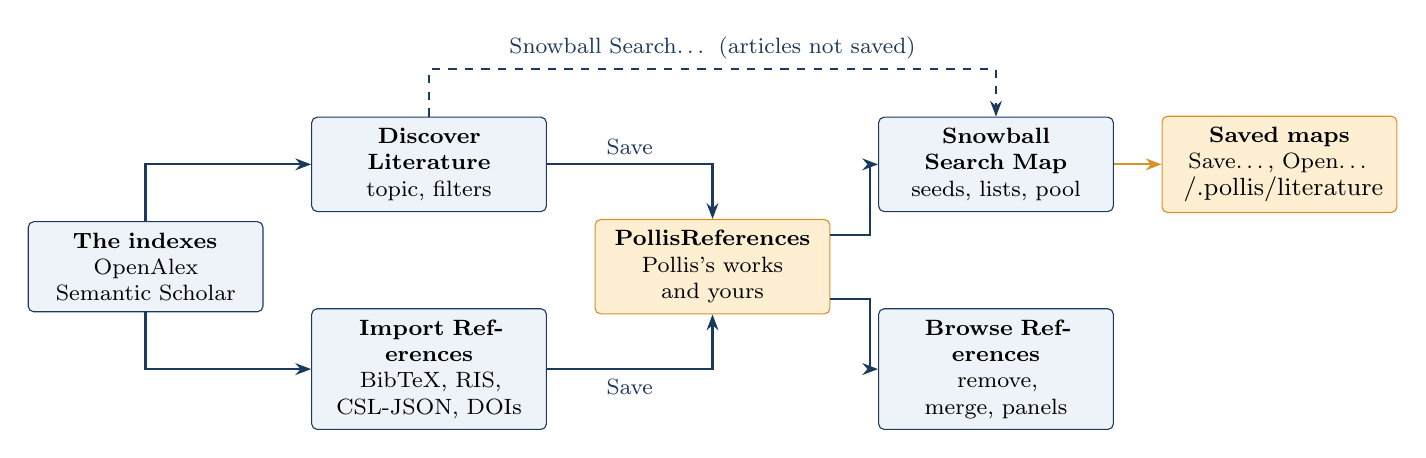
\begin{tikzpicture}[font=\footnotesize,
  box/.style={draw=navy, fill=pale, rounded corners=2pt, align=center, inner sep=4pt, text width=27mm},
  user/.style={box, draw=deepamber, fill=logocream},
  arr/.style={-{Stealth[length=2mm]}, navy, thick}]
  \node[box] (index) at (0, 0) {\textbf{The indexes}\\OpenAlex\\Semantic Scholar};
  \node[box] (discover) at (3.6, 1.3) {\textbf{Discover Literature}\\topic, filters};
  \node[box] (import) at (3.6, -1.3) {\textbf{Import References}\\BibTeX, RIS,\\CSL-JSON, DOIs};
  \node[user] (refs) at (7.2, 0) {\textbf{PollisReferences}\\Pollis's works\\and yours};
  \node[box] (snow) at (10.8, 1.3) {\textbf{Snowball Search Map}\\seeds, lists, pool};
  \node[box] (browse) at (10.8, -1.3) {\textbf{Browse References}\\remove, merge, panels};
  \node[user] (maps) at (14.4, 1.3) {\textbf{Saved maps}\\Save\dots, Open\dots\\\file{~/.pollis/literature}};
  \draw[arr] (index.north) |- (discover.west);
  \draw[arr] (index.south) |- (import.west);
  \draw[arr] (discover.east) -| node[pos=0.25, above] {Save} (refs.north);
  \draw[arr] (import.east) -| node[pos=0.25, below] {Save} (refs.south);
  \draw[arr] (refs.north east) ++(0,-2mm) -| ++(5mm,0) |- (snow.west);
  \draw[arr] (refs.south east) ++(0,2mm) -| ++(5mm,0) |- (browse.west);
  \draw[arr, dashed] (discover.north) -- ++(0,6mm) -| node[pos=0.25, above] {Snowball Search\dots{} (articles not saved)} (snow.north);
  \draw[arr, deepamber] (snow) -- (maps);
\end{tikzpicture}
\end{center}

A search starts at one of the two pages that bring works in. What you keep becomes yours in PollisReferences, beside the
works Pollis cites; Browse References looks after it, and the Snowball Search Map grows a search from it, or from articles
of Discover Literature you have not saved.

\section{The two indexes}\label{sec:indexes}

\subsection{OpenAlex}
A free, open catalogue of scholarly works, the successor of Microsoft Academic Graph. Pollis asks it for most things:
each work's record, its citation count, the counts of the last ten years, its field-weighted citation impact (FWCI), its
citation percentile against works of the same field and year, its journal's 2-year mean citedness, the works it cites
and the works citing it, and an abstract.

\textbf{Budget.} OpenAlex asks for no key, but without one a network shares a free daily budget, about 100 searches a
day. With a key of your own, which OpenAlex gives free, you have a budget of your own. When the budget is used up the
page says so and the search stops; it is not retried.

\subsection{Semantic Scholar}
The Allen Institute for AI's index. Pollis asks it for its own citation count, its \emph{influential} citations (those
that build on a work, not only mention it), its recommendations of related works, and, for a citation, the sentences
that make it and why: background, method or result.

\textbf{Rate.} Without a key, Semantic Scholar answers at a shared rate and is often busy; a key of your own has a rate of
its own. When it is busy, Discover Literature retries the search in the background and shows the OpenAlex rows meanwhile.

\subsection{Keys}
Each index has a \textbf{Set Key} button, \textbf{Change Key} once a key is set, and \textbf{Get a Free Key}, which opens
the index's page for one in the internal browser. A key is kept in the system keychain (Pollis's secret storage), never in
a file; saving an empty key forgets it. The same keys serve every page that asks the index.

\section{Discover Literature}\label{sec:discover}

\subsection{The search}
\begin{center}\small
\renewcommand{\arraystretch}{1.2}
\begin{tabularx}{\linewidth}{@{}p{0.27\linewidth}L@{}}
\toprule
\textbf{Control} & \textbf{What it does}\\
\midrule
Topic, Search In & the words sought, in the title and abstract, or in the title only\\
Index & OpenAlex, Semantic Scholar, or both\\
Field & an OpenAlex field; for Semantic Scholar, the broader field of study it falls in\\
Years From, To & the years of publication\\
Citations At Least & the fewest citations a work may have\\
Recent Citations In the Last & N years, up to 10, this year included: a column, not a filter\\
Influence & Any, Top 10\% or Top 1\% of its field and year (OpenAlex's percentile)\\
Journal Ranking & 2-Year Mean Citedness Above; Norwegian Level 2; Level 1 or 2; SJR Q1; SJR Q1 or Q2\\
Only Articles Anyone Can Read & open access only\\
\bottomrule
\end{tabularx}
\end{center}

The kinds of work listed are articles, reviews, conference papers, preprints, working papers, books and chapters;
editorials, letters and news are left out. The Norwegian levels come from PollisJournals; the SJR quartiles need the
SCImago metrics imported first (right-click PollisJournals in the Databases view, Import Journal Metrics\dots).

\subsection{Two lists made one}
Each index lists its \textbf{200 most cited} works that pass the filters: one request each, since a request of 200 costs
the same as one of 25. The two lists are merged by DOI, or, for a work neither has a DOI for, by its title and first
author. A filter only OpenAlex knows (influence, citedness) cannot be checked for a work only Semantic Scholar found: such
a work is dropped, unless it is a version of a work OpenAlex listed.

\subsection{Versions, never added up}
An index often keeps the versions of one work apart: a preprint, a working paper, a repository copy, the published
article. Each is a row of its own, grouped under the most cited and shown as \emph{+N versions}. Their counts are never
added up, because the indexes count some citations twice across versions; the row shows the counts of its own record.

\subsection{The columns}
\begin{center}\small
\renewcommand{\arraystretch}{1.2}
\begin{tabularx}{\linewidth}{@{}p{0.27\linewidth}L@{}}
\toprule
\textbf{Column} & \textbf{Meaning}\\
\midrule
OpenAlex: Since Publishing & all citations OpenAlex counts\\
OpenAlex: Last N Years & citations in the last N years, from OpenAlex's counts by year\\
FWCI & citations against the average of works of the same field, year and kind (1 is average)\\
Percentile & the work's citation percentile against its field and year\\
Semantic Scholar: Since Publishing & all citations Semantic Scholar counts\\
Influential & Semantic Scholar's influential citations\\
Journal tag & the journal's Norwegian level, 2-year mean citedness and SJR quartile\\
\bottomrule
\end{tabularx}
\end{center}

The table is sorted by the larger of the two counts at first; a heading sorts by its column, clicked again the other way.
Previous, \emph{Page X of Y} and Next page through it. A row opens to show the abstract, from OpenAlex or Semantic Scholar,
with the words of the topic marked.

\textbf{Reconcile Sources} asks each index for the counts of the works only the other found, so that both columns are
filled.

\subsection{What to do with the works ticked}
\begin{center}\small
\renewcommand{\arraystretch}{1.2}
\begin{tabularx}{\linewidth}{@{}p{0.27\linewidth}L@{}}
\toprule
\textbf{Action} & \textbf{What it does}\\
\midrule
Save to PollisReferences & writes each as your work, with its versions and today's counts (\S\ref{sec:files})\\
Copy BibTeX & the entries, to the clipboard\\
Open PDFs & each open copy in the internal browser; a site that turns it away, as IEEE Xplore does, is avoided for a free copy elsewhere when there is one\\
Show in Panel\dots & a chooser of the panels with References, searchable, each saying how many works it cites; saved only when you confirm\\
See in References & opens Browse References at the works\\
Snowball Search\dots & opens the Snowball Search Map with the works as seeds, saved or not\\
$\times$ & removes a row from the table, not from anything saved\\
\bottomrule
\end{tabularx}
\end{center}

The works you keep stay kept when the page is closed and opened again.

\section{Import References}\label{sec:import}

\subsection{Bringing them in}
\textbf{Paste} takes text; \textbf{Files} takes one or more files (Choose Files\dots). The format is told from the text:
BibTeX or BibLaTeX, RIS, CSL-JSON, or a list of DOIs, one a line.

\subsection{Looking them up}
\textbf{Look Up in OpenAlex and Semantic Scholar} finds each reference in the indexes: by DOI, 100 to a request, or else by
title, one request each. The file's fields are kept; OpenAlex fills the fields the file lacks and brings the counts and
versions. Each row then says what happened: \emph{Found in OpenAlex by DOI}, \emph{by title}, \emph{Not found} or
\emph{Not looked up}.

\subsection{Ticks}
The links above the table tick All, None, Found, Not Found, Not Looked Up or Not Yet Saved. \textbf{Look Up Ticked} looks up
again only those; \textbf{Remove Unticked\dots} drops the others from the page, after asking. The actions of Discover
Literature (\S\ref{sec:discover}) work on the ticked rows.

\subsection{Keys of imported works}
A work saved from an import keeps its DOI as its id; a work without one is given \file{import:} and a hash of its title,
year and first author, so importing the same file twice does not make two works. Its BibTeX key is made as Pollis makes
every key, from the first author and the year, with a letter for the next free one.

\section{Browse References}\label{sec:browse}

Every work in PollisReferences: those Pollis cites and ships, those you saved or added to a panel, and your corrections of
Pollis's works. Search looks in the title, authors, venue and key; \textbf{Show} narrows to All, User, Corrected or
Built-in. The columns are Year, Work, Key, Citations (the latest count of each index, dated), In Panels, and Records (the
versions in the indexes). Headings sort; a pager pages.

\begin{center}\small
\renewcommand{\arraystretch}{1.2}
\begin{tabularx}{\linewidth}{@{}p{0.27\linewidth}L@{}}
\toprule
\textbf{Action} & \textbf{What it does}\\
\midrule
Remove & a work of yours, with its versions and counts, and off the panels you showed it in\\
Undo Correction & returns a work of Pollis to how Pollis has it\\
Show in Panel\dots & as in Discover Literature\\
Possible Duplicates & works with the same first author, years at most two apart, and titles alike or one the other with a subtitle\\
Merge\dots & of two works, keeps one's details, under the key that sorts first; the other's key becomes an alias, shown as \emph{Also cited as}, and its OpenAlex record a version of the work kept\\
Undo Merge & parts them again\\
\bottomrule
\end{tabularx}
\end{center}

Pollis's own works cannot be removed, only corrected; a correction is a work of yours with Pollis's key, and Undo
Correction removes it.

\section{Snowball Search Map}\label{sec:snowball}

Snowballing is the oldest way through a literature: from a few works you trust, the \emph{seeds}, follow the works that
cite them (forward) and the works they cite (backward), and keep the works many seeds lead to. The map does that with the
indexes and keeps a record of every step.

\subsection{Seeds}
Seeds come from Discover Literature (Snowball Search\dots), saved there or not, or from \textbf{Add Seeds}, which finds
works of PollisReferences by title, author or key. On the map the seeds are pills, E1, E2\dots; where they came from is a
dashed source box. Clicking a seed chooses it (filled): the next list follows only the seeds chosen, and \textbf{All Seeds}
follows all again. $\times$ removes a seed: it stays on the map, dashed, and no longer counts.

\subsection{Lists}
Each list is a box, L1, L2\dots, with how many works it brought and how many were new to the pool.
\begin{center}\small
\renewcommand{\arraystretch}{1.2}
\begin{tabularx}{\linewidth}{@{}p{0.18\linewidth}L@{}}
\toprule
\textbf{Edge} & \textbf{What is listed}\\
\midrule
Cited By & the works citing each seed, as OpenAlex has them: the 2,000 most cited, ten requests of 200\\
Cites & the works each seed cites, as OpenAlex has them\\
Related & up to 500 works Semantic Scholar recommends for each seed by the likeness of their texts, looked up in OpenAlex 50 to a request; for a seed Semantic Scholar does not know, OpenAlex's related works (about ten). Marked $\approx$, and not counted in Links\\
\bottomrule
\end{tabularx}
\end{center}

\textbf{Select} on the edge bar picks seeds instead of following; \textbf{Landscape} or \textbf{Portrait} lays the map
out with each step a column further, or a row further.

\subsection{The pool and its ranking}
Every work of every list goes into one pool. It is ranked by \textbf{Links}, the number of seeds (still counted) the work is
tied to by Cited By or Cites, then by its citations; a work you excluded comes after all the others. The \textbf{top} is
the first 20. The \textbf{From} column names the lists a work is in; \textbf{Show} narrows the pool to All, one list, New
Since Last Step, or Candidates (the works of the top that are neither seeds nor excluded). \textbf{Seed} makes a work of
the pool a seed; \textbf{Exclude} keeps it out of the top, \textbf{Include} lets it back.

A line under the pool tells where the search stands: \emph{\{n\} works from L1--L2, the last step added \{k\}, \{j\} of
them in the top 20}.

\subsection{How the citations are made}
\textbf{Ask Semantic Scholar About the Citations} (a tick, remembered) asks, for each list of citations, how each work
cites each seed: up to 1,000 citations a request, ten requests a seed at most. A work's Links cell then shows a dot per
seed, filled when the citation is influential; opening it shows, seed by seed, the intents (Background, Method, Result)
and the sentences. Among works tied to as many seeds, those with more influential citations rank first when sorted by
Links. A work Semantic Scholar has no record of, or that has no DOI to ask by, is marked so.

\subsection{Rounds and saturation}
A \emph{round} is a set of works made seeds, then the lists of citations that follow them. Each list of citations keeps
the pool's top as it was after it, and the next round is compared with it: a line per round tells how many works of the
top are new, marked $\uparrow$ \emph{New} in the top 20. A round that brings nothing new into the top has
\textbf{saturated} the search, and the page says \emph{The search has saturated}.

\textbf{Run to Saturation} runs the rounds itself: it follows the seeds not followed yet, then, round after round, makes the
best candidates seeds and follows them, until the search saturates or the rounds run out. Beside it:
\begin{itemize}
  \item \textbf{Seeds a round}, 5 at first: the candidates made seeds each round;
  \item \textbf{Rounds at most}, 6 at first;
  \item \textbf{Following}: Cited By, Cites, or both.
\end{itemize}
They are remembered. While it runs its button reads \textbf{Stop}, which ends the run once the round it is in ends; a list
half fetched is never kept, so a step is always whole. Excluding a work keeps Run to Saturation from making it a seed.

\subsection{Saving and opening maps}
\textbf{Save\dots} writes the map under a name in \file{~/.pollis/literature}: a TOML record of its steps, and a DuckDB
file of its works beside it (\S\ref{sec:files}); a map of the same name is replaced only after asking. \textbf{Open\dots}
lists the maps saved, the latest first. \textbf{New Search} empties the map, after warning when it has steps not saved.
The map in the page is kept while the window is open, the page closed or not.

\subsection{When something goes wrong}
\begin{itemize}
  \item \textbf{The budget is used up}: OpenAlex's free budget for the day is spent. Set a key of your own, or wait until
    tomorrow; the steps taken are kept.
  \item \textbf{The index could not be reached}: no connection, or the index is down. The step is not kept; take it again.
  \item \textbf{No record}: an index does not know the seed. Cited By and Cites need OpenAlex's record (found by DOI, or by
    title and first author); Related falls back on OpenAlex when Semantic Scholar has none.
\end{itemize}

\section{What is written, and where}\label{sec:files}

\subsection{Your references}
What the pages keep is yours, in JSON Lines files that no update of Pollis touches. They are appended to, never rewritten:
a change is a new line, and for each key the last line wins.
\begin{center}\small
\renewcommand{\arraystretch}{1.2}
\begin{tabularx}{\linewidth}{@{}p{0.36\linewidth}L@{}}
\toprule
\textbf{File in \file{~/.pollis/references}} & \textbf{What a line is}\\
\midrule
\file{references.jsonl} & a work you saved or imported, or a correction of one of Pollis's; a removal (\file{removed}), or a merge (the key it was merged into)\\
\file{versions.jsonl} & a record of a work in an index: published, preprint, working paper or repository\\
\file{counts.jsonl} & a citation count of a version, with the index and the date it was seen\\
\file{panels.jsonl} & a work shown in, or hidden from, the References of a panel\\
\bottomrule
\end{tabularx}
\end{center}

At the next start of the Julia REPL, PollisDB builds the PollisReferences database over these files and Pollis's works:
\file{all_references}, \file{all_counts} and \file{all_versions} (see \emph{Drill-down: Data Packages}). The pages
themselves read the files directly, so what you save shows at once. A key is never given twice, even to a work removed.

\subsection{Your maps}
A saved map is two files of the same name in \file{~/.pollis/literature}:
\begin{itemize}
  \item \file{NAME.toml}, the record: one \file{[[step]]} per action, with its id (E1, L1\dots), what it did (seed, Cited By,
    Cites, Related, removal), where a seed came from, its key or DOI, when (UTC, to the second), and for a list the works
    it brought, the works the index has and the top after it;
  \item \file{NAME.duckdb}, the works: the tables \file{articles} (seeds not in PollisReferences), \file{seeds},
    \file{works}, \file{links} (work, seed, relation, list), \file{contexts} (how a work cites a seed),
    \file{s2\_asked} and \file{excluded}.
\end{itemize}
The map drawn on the page is drawn from the steps alone. While the map is open its tables live in an in-memory DuckDB, in
a process of its own, with PollisReferences attached read-only for the seeds that are your works.

\subsection{Kept by the page}
The articles kept in Discover Literature and the references being imported are remembered by Pollis between sessions, as
are the choices of the Snowball page (Ask Semantic Scholar, the layout, Run to Saturation's settings). They are not your
data: clearing them loses nothing saved.

\section{Where things are}\label{sec:where}

\begin{center}\small
\renewcommand{\arraystretch}{1.2}
\begin{tabularx}{\linewidth}{@{}p{0.47\linewidth}L@{}}
\toprule
\textbf{File} & \textbf{Role}\\
\midrule
\file{.../compose/browser/compose.contribution.ts} & The Literature Radar menu\\
\file{.../compose/browser/literatureRadarPage.ts} & Discover Literature and Import References\\
\file{.../compose/browser/browseReferencesPage.ts} & Browse References\\
\file{.../compose/browser/snowballSearchPage.ts} & Snowball Search Map: steps, rounds, ranking, saving\\
\file{.../compose/common/snowballSearch.ts} & Its command, the seeds other pages give it, its database service\\
\file{.../compose/node/snowballDatabaseMain.ts} & The map's DuckDB process\\
\file{.../model/browser/common/referenceLibrary.ts} & PollisReferences in TypeScript: the user's JSON Lines files, keys, BibTeX\\
\file{.../terminalserver/PollisDB.jl} & \file{build\_references}: the PollisReferences database\\
\file{docs/guide/pollis\_guide.tex} & The Guide's Literature Radar and Snowball sections\\
\bottomrule
\end{tabularx}
\end{center}

\section{Open points}\label{sec:open}
\begin{itemize}
  \item \textbf{Counts age}: the counts saved are those of the day they were saved; nothing refreshes them on its own.
  \item \textbf{One index for citations}: Cited By and Cites follow OpenAlex only; Semantic Scholar's lists are asked only
    for how the citations are made.
  \item \textbf{Saturation is of the top}: a round that changes nothing in the top 20 saturates the search, even when it
    adds works further down.
\end{itemize}

\end{document}
